\documentclass[10pt]{scrartcl}
\usepackage[utf8]{inputenc}
%teoremi
\usepackage{amsmath,amssymb,amsthm}
\usepackage[croatian]{babel}
\usepackage[unicode]{hyperref}
%za teoreme, def, prop, kor, itd
\usepackage{thmtools}
\declaretheorem{teorem}
%analogno se moze dodati napomena (style=remark) i slično
%ako se makne sibling, onda neovisno kreće brojač za broj tog npr zadatka, ovako je sve namješteno na isti brojač
\declaretheorem[sibling=teorem]{korolar}
\declaretheorem[sibling=teorem]{propozicija}
\declaretheorem[style=definition,sibling=teorem]{definicija}
%za algoritme
\usepackage{algorithm,algorithmic,lipsum}
\usepackage{mathtools}
\usepackage[T1]{fontenc}
\usepackage[table,xcdraw]{xcolor}
\usepackage{tabularx}
\usepackage{textcomp}
\usepackage{graphicx}

%ode možete renew command za algoritmne, dobro bi bilo trenutne ne dirati, jer su postavljeni kako je meni zasad odgovaralo. ako minjate, onda bacite oko na postojece algoritme, td ne utjece na njih
\newenvironment{croatianalgorithm}[1][]
  {\begin{algorithm}[#1]
     \selectlanguage{croatian}%
     \floatname{algorithm}{Algoritam}%
     \renewcommand{\algorithmicif}{\textbf{ako}}%
     \renewcommand{\algorithmicthen}{\textbf{onda}}%
     \renewcommand{\algorithmicend}{\textbf{kraj}}%
     \renewcommand{\algorithmicwhile}{\textbf{sve dok}}%
     \renewcommand{\algorithmicdo}{\textbf{ponavljaj}}%
     \renewcommand{\algorithmicreturn}{\textbf{vrati}}%
     \renewcommand{\algorithmicendwhile}{\textbf{kraj sve dok}}%
     \renewcommand{\algorithmicfor}{\textbf{za svaki}}
     \renewcommand{\algorithmicendfor}{\textbf{kraj za svaki}}%
     % Set other language requirements
  }
  {\end{algorithm}}
%za slike
\usepackage{graphicx}


\begin{document}

\begin{titlepage}
	\centering
	
\includegraphics[width=0.3\textwidth]{pmf}\par\vspace{1cm}
	{\scshape NAPREDNE BAZE PODATAKA \\ projektni zadatak \par}
	\vspace{1cm}
	{\huge\bfseries Primjena algoritama za pretraživanje grafova i pronalazak puta na grafovskoj bazi podataka u Neo4j \par}
	\vspace{5cm}
	{\Large\itshape TIM THETA\par
	\vspace{0.2cm}
	{\Large\itshape Petra Škrabo}\par
	\vspace{0.1cm}
	{\Large\itshape Ivan Štruklec}\par
	\vspace{0.1cm}
	{\Large\itshape Katarina Šupe}\par
	\vspace{0.1cm}
	{\Large\itshape Mateja Terzanović}\par
	\vspace{0.1cm}
	{\Large\itshape Margarita Tolja}\par
	\vfill}
\end{titlepage}

\tableofcontents
\newpage
\section{Uvod}

\begin{figure}[H]
    \centering
    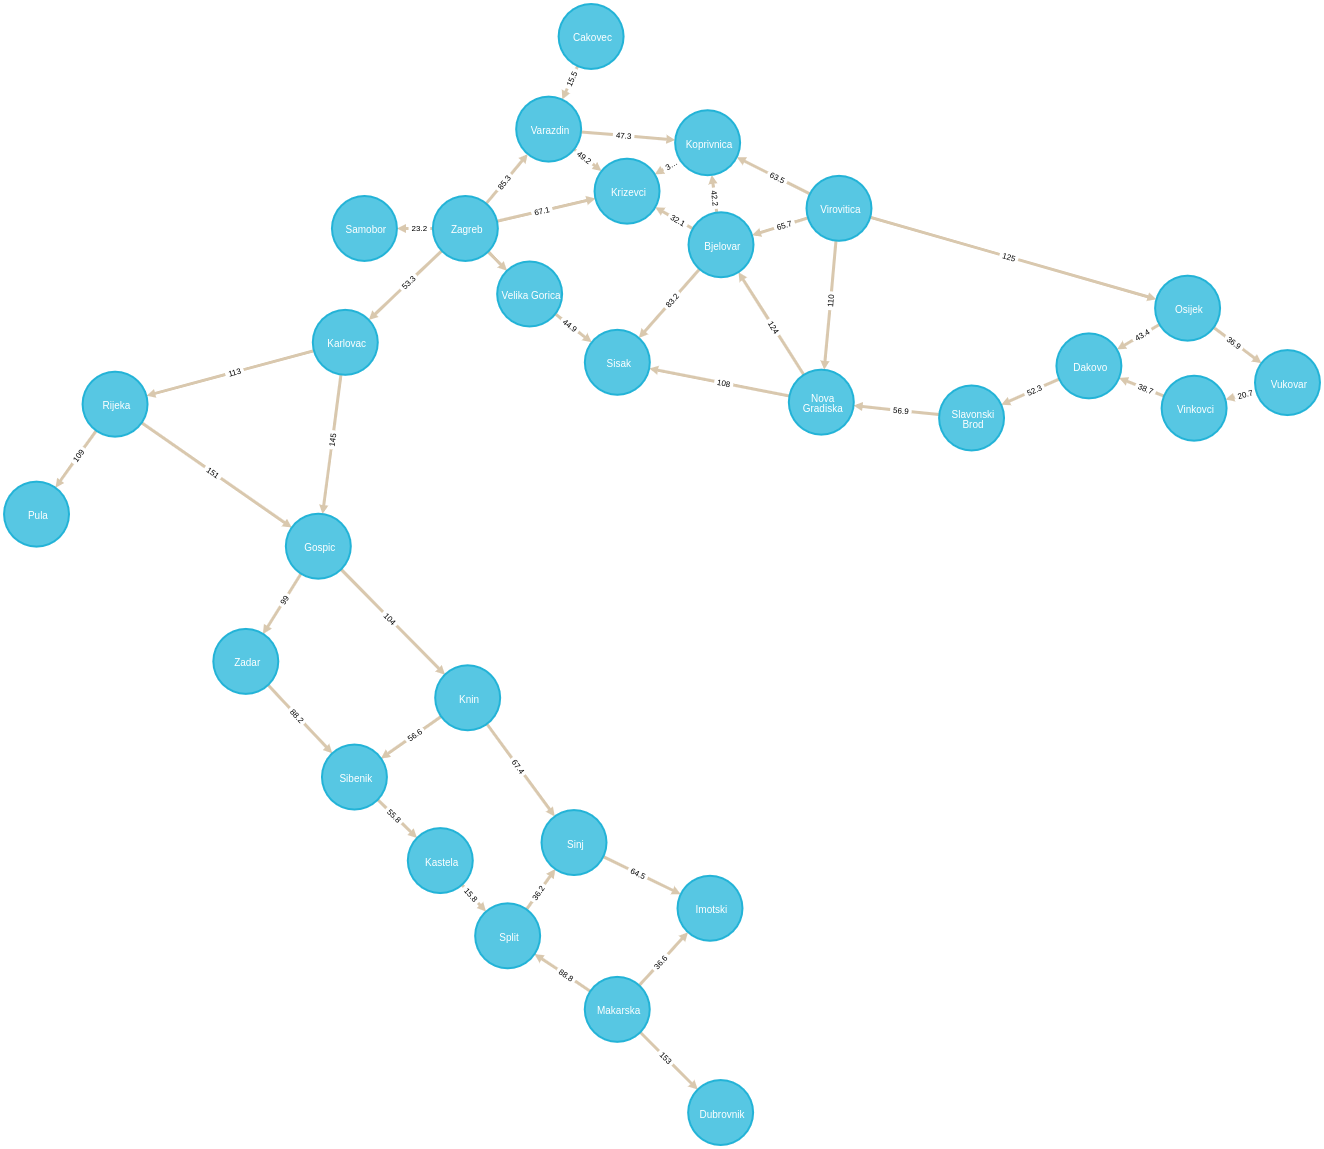
\includegraphics[scale=0.3]{graph}
    \caption{Grafovska baza odabranih hrvatskih gradova}
    \label{fig:baza}
\end{figure}


\pagebreak[2]

\section{Najkraći put}

Algoritmi traženja najkraćeg puta u težinskom grafu
pronalaze put koji spaja dva promatrana vrha s najmanjim
mogućim zbrojem težina bridova na tom putu. Glavni
algoritam za rješavanje problema ove vrste je
\emph{Dijkstrin algoritam} koji je ujedno implementiran
i u standardnoj \emph{shortestPath} funkciji za
pronalazak najkraćeg puta Neo4j \emph{Graph Algorithms}
biblioteke. Postoje i dvije tehnike ubrzanja Dijkstrinog
algoritma, \emph{dvosmjerni Dijkstrin algoritam} i
\emph{algoritam $A^*$}, no mi ćemo se bazirati na
općenitu verziju.

\subsection{Dijkstrin algoritam}

Osnovna ideja algoritma je iterativno računanje najkraćeg puta krenuvši od početnog čvora tako da se svakom iteracijom ažurira udaljenost puta do trenutno promatranog čvora sve dok ne obiđe sve čvorove.

Za bolje razumijevanje prvo navodimo pseudokod algoritma, a zatim njegov detaljniji opis.

\begin{croatianalgorithm}[H]
  \caption{Dijkstrin algoritam}
  \begin{algorithmic}[1]
    \FOR{vrh $v$ u grafu}
        \STATE udaljenost[$v$] $\coloneqq  \infty$
        \STATE posjećen[$v$] $\coloneqq$ nedefinirano
    \ENDFOR 
    \item[]
    \STATE udaljenost[početni\_vrh] $\coloneqq 0$
    \STATE $Q \coloneqq$ skup svih vrhova u grafu
    \item[]
    \WHILE{$Q$ nije prazan skup}
        \STATE $u \coloneqq$ vrh $v \in Q$ sa najmanjom udaljenosti \emph{udaljenost$[v]$}
        \STATE ukloni $u$ iz $Q$
        \FOR{susjed $v$ od $u$}
            \STATE putanja $\coloneqq$ udaljenost[$u$] + udaljenost\_između($u,v$)
            \IF{putanja < udaljenost[$v$]}
                \STATE udaljenost[$v$] $\coloneqq$ putanja
                \STATE posjećen[$v$] $\coloneqq u$
            \ENDIF
        \ENDFOR
    \ENDWHILE
    \item[]
    \RETURN udaljenost[\,], posjećen[\,]
  \end{algorithmic}
\end{croatianalgorithm}


\emph{Udaljenost$[v]$} čuva najkraću udaljenost vrha $v$ od početnog vrha i predstavlja akumulirane težine između ta dva vrha, a \emph{posjećen$[v]$} čuva informaciju o posjećenosti vrha~$v$.

Na početku se svaki vrh $v$ označava kao neposjećen, a njegova \emph{udaljenost$[v]$} postavlja na beskonačnu vrijednost. Iznimno, udaljenost ishodišnog vrha postavlja se na nulu.
U skup $Q$ stavljaju se svi vrhovi grafa, budući da još niti jedan nije obrađen.

Sljedeći korak je pretražiti cijeli graf i za svaki vrh iz grafa odrediti njegovu udaljenost od početnog vrha tako da ona bude najmanja moguća.
Prvo se određuje onaj vrh $u$ čija je \emph{udaljenost$[u]$} najmanja. Vidimo da će se u prvom koraku obraditi početni vrh budući da je njegova udaljenost nula, dok su sve druge udaljenosti postavljene na beskonačnu vrijednost.
Nakon odabira vrha on se briše iz skupa $Q$. Algoritam ga zatim obrađuje na način da se \emph{udaljenost$[v]$} svakog njegovog susjeda $v$ ažurira ukoliko se on još uvijek nalazi u skupu $Q$ i ako je dobivena \emph{udaljenost$[v]$} preko promatranog čvora manja nego ona koju je $v$ imao do tada. Ažuriranje se radi određivanjem zbroja udaljenosti između susjednog vrha i vrijednosti trenutno promatranog vrha. Ako se susjedni vrh ne nalazi u $Q$ to znači da ga je algoritam već obradio, odnosno da je njegova udaljenost najmanja moguća. 

Kad se svi susjedi promatranog vrha obrade on se označava kao posjećen i algoritam nastavlja s obradom sljedećeg vrha, onog s trenutno najmanjom udaljenosti od početnog vrha.

%\medskip
Nakon završetka algoritma \emph{posjećen} će imati strukturu koja zapravo podgraf orginalnog grafa i predstavlja najkraći put između početnog vrha i svih drugih vrhova. 
%\bigskip

Važno je napomenuti da Dijkstrin algoritam rješava problem najkraćeg puta u grafu s pozitivnim težinama bridova.

\subsection{Primjena Dijkstrinog algoritma na promatranu bazu}

U našem slučaju su težinama reprezentirane udaljenosti pa nam pozitivnost neće predstavljati problem. Pogledamo li napravljenu grafovsku bazu primjećujemo grad Zagreb kao veliko prometno čvorište. Uzmimo njega kao početni čvor i provedimo Dijkstrin algoritam. Znamo da ćemo kao rezultat dobiti najkraći put od Zagreba do svakog grada iz promatrane baze.

%\medskip
Prvo ćemo provesti algoritam „ručno”.

Inicijalna udaljenost Zagreba je nula, dok su udaljenosti svih ostalih gradova promatrane baze postavljene na beskonačnu vrijednost. 
Dakle, prvo se obrađuje vrh Zagreb. Njegovi susjedni vrhovi su Velika Gorica~(18.7), Samobor~(23.2), Karlovac~(53.3), Križevci~(67.1) i Varaždin~(85.3). 

Vrh s najmanjom udaljenošću je Velika Gorica pa je upravo ona sljedeći vrh koji ćemo promatrati. Zagreb označavamo kao posjećen.
Jedini susjed od Velike Gorice je Sisak čija se udaljenost od Zagreba postavlja na 63.6. Velika Gorica se označava kao posjećeni vrh.

Sljedeći vrh najbliži Zagrebu je Samobor~(23.2). On nema susjeda, pa u ovom koraku samo Samobor svrstavamo među posjećene vrhove.
Karlovac~(53.3) trenutno je vrh s najmanjom udaljenošću pa promatramo njegove susjede Rijeku~(166.3) i Gospić~(198.3), a Karlovac označavamo ga kao posjećen.

U sljedećoj iteraciji algoritam za promatrani vrh uzima Sisak~(63.6), a njegove susjede označava vrijednostima Bjelovar~(146.8), Nova Gradiška~(171.6). 
Sisak označava kao posjećen.

Početnom vrhu sada su najbliži Križevci~(67.1). Njegovi susjedni vrhovi su Bjelovar~(99.2), Koprivnica~(99.3) i Varaždin~(116.3). U ovoj iteraciji algoritam Varaždinu ne ažurira udaljenost budući da je u Varaždin bliže stići iz Zagreba za 85.3 kilometara, nego preko Križevaca za 116.3 kilometara. Križevci su sada posjećeni.

Na isti način nastavljamo provoditi algoritam sve dok svi gradovi nisu označeni kao posjećeni. Tada algoritam završava, a najkraći put iz Zagreba do svakog pojedinog grada iščitavamo iz koraka algoritma. Detaljna provedba algoritma prikazana je u ----- tablici.

\pagebreak[4]
\begin{center}
\begin{table}[H]
\caption{Koraci Dijkstrinog algoritma sa Zagrebom kao početnim čvorom}
\begin{tabularx}{1\textwidth}{c X c}
\hline
\textbf{Trenutni vrh} & \textbf{Susjedni (neposjećen)}                                                          & \textbf{Prethodno posjećen} \\ \hline
\textbf{Zagreb (0)}             & Velika Gorica (18.7), Samobor (23.2), Karlovac~(53.3), Križevci (67.1), Varaždin (85.3) & X                           \\ \hline
Velika Gorica (18.7)   & Sisak (63.6)                                                                            & Zagreb                      \\ \hline
Samobor (23.2)         & X                                                                                       & Velika Gorica               \\ \hline
Karlovac (53.3)        & Rijeka (166.3), Gospić (198.3)                                                          & Samobor                     \\ \hline
Sisak (63.6)           & {\color[HTML]{9B9B9B} Bjelovar (146.8)}, Nova Gradiška (171.6)                          & Karlovac                    \\ \hline
Križevci (67.1)        & Bjelovar (99.2), Koprivnica (99.3), {\color[HTML]{9B9B9B} Varaždin~(116.3)}             & Sisak                       \\ \hline
Varaždin (85.3)        & Čakovec (100.8), {\color[HTML]{9B9B9B} Koprivnica (132.6)}                              & Križevaci                   \\ \hline
Bjelovar (99.2)        & {\color[HTML]{9B9B9B} Nova Gradiška (223.2), Virovitica (164.9), Koprivnica~(141.4)}    & Varaždin                    \\ \hline
Koprivnica (99.3)      & Virovitica (162.8)                                                                      & Bjelovar                    \\ \hline
Čakovec (100.8)        & X                                                                                       & Koprivnica                  \\ \hline
Virovitica (162.8)     & {\color[HTML]{9B9B9B} Nova Gradiška (272.8)}, Osijek (287.8)                            & Čakovec                     \\ \hline
Rijeka (166.3)         & Pula (275.3), {\color[HTML]{656565} Gospić (317.3)}                                     & Virovitica                  \\ \hline
Nova Gradiška (171.6)  & Slavonski Brod (228.5)                                                                  & Rijeka                      \\ \hline
Gospić (198.3)         & Zadar (297.3), Knin (302.3)                                                             & Nova Gradiška               \\ \hline
Slavonski Brod (228.5) & Đakovo (280.8)                                                                          & Gospić                      \\ \hline
Pula (275.3)           & X                                                                                       & Slavonski Brod              \\ \hline
Đakovo (280.8)         & {\color[HTML]{9B9B9B} Osijek (324.2)}, Vinkovci (319.5)                                 & Pula                        \\ \hline
Osijek (287.8)         & Vukovar (324.7)                                                                         & Đakovo                      \\ \hline
Zadar (297.3)          & {\color[HTML]{9B9B9B} Šibenik (385.5)}                                                  & Osijek                      \\ \hline
Knin (302.3)           & Šibenik (358.9), Sinj (369.7)                                                           & Zadar                       \\ \hline
Vinkovci (319.5)       & {\color[HTML]{9B9B9B} Vukovar (340.2)}                                                  & Knin                        \\ \hline
Vukovar (324.7)        & X                                                                                       & Vinkovci                    \\ \hline
Šibenik (358.9)        & Kaštela (414.7)                                                                         & Vukovar                     \\ \hline
Sinj (369.7)           & Imotski (434.2), Split (405.9)                                                          & Šibenik                     \\ \hline
Split (405.9)          & {\color[HTML]{9B9B9B} Kaštela (421.7), Makarska (494.7)}                                & Sinj                        \\ \hline
Kaštela (414.7)        & X                                                                                       & Split                       \\ \hline
Imotski (434.2)        & Makarska (470.8)                                                                        & Kaštela                     \\ \hline
Makarska (470.8)       & Dubrovnik (623.8)                                                                       & Imotski                     \\ \hline
Dubrovnik (623.8)      & X                                                                                       & Makarska                    \\ \hline
X                      & X                                                                                       & Dubrovnik                   \\ \hline
\end{tabularx}
\end{table}
\end{center}

Iz tablice sada lako iščitavamo najkraći put od Zagreba do bilo kojeg grada iz naše mreže gradova čitajući korake unatrag. Bitno je zanemariti gradove označene sivom bojom jer njihovu udaljenost dobivenu tom iteracijom ne ažuriramo, budući da već postoji kraći put od početnog čvora do njega. Osim toga, u stupcu \textbf{trenutni vrh} pokraj svakog grada nalazi se i njegova točna udaljenost od Zagreba. U stupcu \textbf{prethodno posjećen} možemo iščitati sve vrhove posjećene prije trenutnog tako da krenemo od vrha stupca i čitamo vrhove sve do retka koji u prvom stupcu sadrži trenutno posjećen vrh. Po završetku algoritma stupac \textbf{prethodno posjećen} sadrži sve gradove iz promatrane baze.

%bigskip
Primjeri najkraćih puteva od Zagreba do Splita, Rijeke i Osijeka. Čitamo:
\begin{enumerate}
    \item Split\textleftarrow Sinj\textleftarrow Knin\textleftarrow Gospić\textleftarrow Karlovac\textleftarrow Zagreb
    \item Rijeka\textleftarrow Karlovac\textleftarrow Zagreb
    \item Osijek\textleftarrow Virovitica\textleftarrow Koprivnica\textleftarrow Križevci\textleftarrow Zagreb
\end{enumerate}

Ovaj rezultat potvrđuje i \emph{Cypher} pozivanjem \emph{shortestPath} funkcije iz biblioteke s graf algoritmima.

\begin{table}[H]
\centering
\caption{Tablica udaljenosti najkraćeg puta od Zagreba do Splita}
\begin{tabular}{|l|l|}
\hline
\textbf{name} & \textbf{cost}      \\ \hline
"Zagreb"      & 0.0                \\ \hline
"Karlovac"    & 53.3               \\ \hline
"Gospic"      & 198.3              \\ \hline
"Knin"        & 302.3              \\ \hline
"Sinj"        & 369.70000000000005 \\ \hline
"Split"       & 405.90000000000003 \\ \hline
\end{tabular}
\end{table}

\begin{figure}[H]
    \centering
    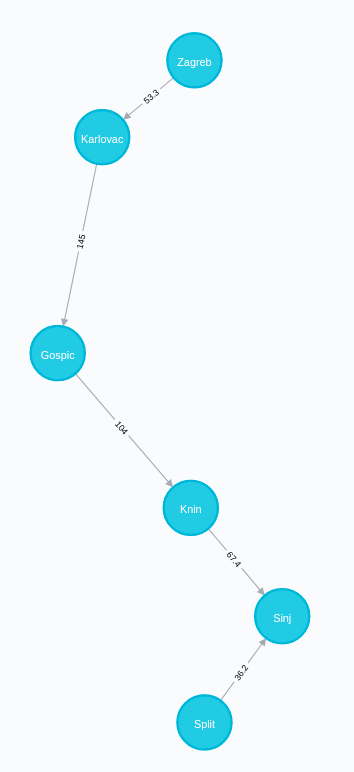
\includegraphics[scale=0.25]{zg-st}
    \caption{Najkraći put od Zagreba do Splita}
\end{figure}

\begin{table}[H]
\centering
\caption{Tablica udaljenosti najkraćeg puta od Zagreba do Rijeke}
\begin{tabular}{|l|l|}
\hline
\textbf{name} & \textbf{cost} \\ \hline
"Zagreb"      & 0.0           \\ \hline
"Karlovac"    & 53.3          \\ \hline
"Rijeka"      & 166.3         \\ \hline
\end{tabular}
\end{table}

\begin{figure}[H]
    \centering
    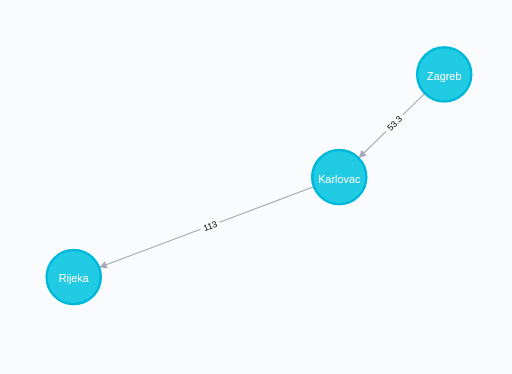
\includegraphics[scale=0.4]{zg-ri}
    \caption{Najkraći put od Zagreba do Rijeke}
\end{figure}


\begin{table}[H]
\centering
\caption{Tablica udaljenosti najkraćeg puta od Zagreba do Osijeka}
\begin{tabular}{|l|l|}
\hline
\textbf{name} & \textbf{cost} \\ \hline
"Zagreb"      & 0.0           \\ \hline
"Krizevci"    & 67.1          \\ \hline
"Koprivnica"  & 99.3          \\ \hline
"Virovitica"  & 162.8         \\ \hline
"Osijek"      & 287.8         \\ \hline
\end{tabular}
\end{table}

\begin{figure}[H]
    \centering
    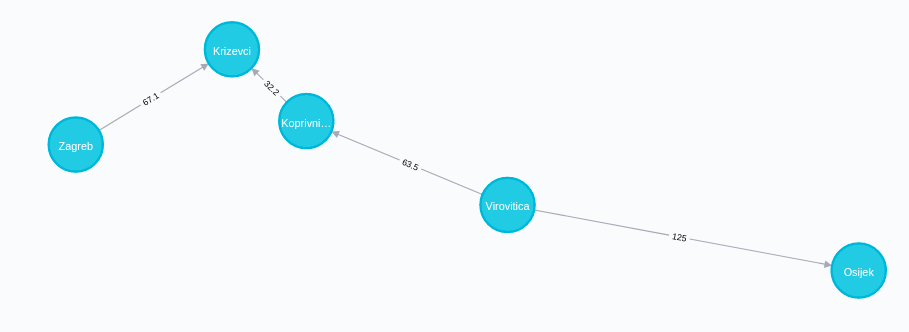
\includegraphics[scale=0.3]{zg-os}
    \caption{Najkraći put od Zagreba do Osijeka}
\end{figure}


Do sada smo promatrali izvornu verziju algoritma, ali ona se lako može modificirati tako da algoritam pronalazi najkraći put između dvaju zadanih vrhova zaustavljajući se nakon što je najkraći put iz početnog do krajnjeg vrha određen. Dakle, proces ažuriranja susjednih vrhova u prethodno opisanom algoritmu se zaustavlja u trenutku kad se krajnji vrh označi kao posjećen.


\subsection{Računanje udaljenosti između dvaju gradova Dijkstrinim algoritmom}

Za primjer uzmimo pronalazak najkraćeg puta iz početnog vrha Zadra i krajnjeg vrha Bjelovara. Iteracije kojima ovaj algoritam dolazi do rješenja prikazane su u sljedećoj tablici, a postupak je jednak prethodno opisanom izuzev provjere je li vrh koji je trenutno posjećen jednak krajnjem vrhu.


\begin{center}
\begin{table}[H]
\caption{Koraci Dijkstrinog algoritma za put od Zadra do Bjelovara}
\begin{tabularx}{1\textwidth}{c X c}
\hline
\textbf{Trenutni čvor}                           & \textbf{Susjedni (neposjećen)}                                                      & \textbf{Prethodno posjećen} \\ \hline
{\textbf{Zadar (0)}}        & Šibenik (88.2), Gospić (99)                                                         & X                           \\ \hline
Šibenik (88.2)                                   & Kaštel (144), Knin (144.8)                                                          & Zadar                       \\ \hline
Gospić (99)                                      & {\color[HTML]{9B9B9B} Knin (203)}, Karlovac (244), Rijeka (250)                     & Šibenik                     \\ \hline
Kaštel (144)                                     & Split (159.8)                                                                       & Gospić                      \\ \hline
Knin (144.8)                                     & {\color[HTML]{9B9B9B} Sinj (212.2)}                                                 & Kaštel                      \\ \hline
Split (159.8)                                    & Sinj (196), Makarska (248,6)                                                        & Knin                        \\ \hline
Sinj (196)                                       & Imotski (260.5)                                                                     & Split                       \\ \hline
Karlovac (244)                                   & Zagreb (297,3), Rijeka (357)                                                        & Sinj                        \\ \hline
Makarska (248.6)                                 & {\color[HTML]{9B9B9B} Imotski (285,2)}, Dubrovnik (401.6)                           & Karlovac                    \\ \hline
Rijeka (250)                                     & Pula (539)                                                                          & Makarska                    \\ \hline
Imotski (260)                                    & X                                                                                   & Rijeka                      \\ \hline
Zagreb (297.3)                                   & Velika Gorica (316), Samobor (320.5), Križevci (364.4), Varaždin (382.6)            & Imotski                     \\ \hline
Velika Gorica (316)                              & Sisak (360.9)                                                                       & Zagreb                      \\ \hline
Samobor (320.5)                                  & X                                                                                   & Velika Gorica               \\ \hline
Pula (359)                                       & X                                                                                   & Samobor                     \\ \hline
Križevci (364.4)                                 & Bjelovar (396.5), Koprivnica (396.6), {\color[HTML]{9B9B9B} Varaždin (413.6)}       & Pula                        \\ \hline
Sisak (360.9)                                    & {\color[HTML]{9B9B9B} Bjelovar (444.1)}, Nova Gradiška (468.9)                      & Križevaci                   \\ \hline
Varaždin (382.6)                                 & Čakovec (398.1), {\color[HTML]{9B9B9B} Koprivnica(429,9)}                           & Sisak                       \\ \hline
{\textbf{Bjelovar (396.5)}} & {\color[HTML]{9B9B9B} Koprivnica (438,7), Virovitica (462.2),  Nova Gradiška (520)} & Varaždin  
\end{tabularx}
\end{table}
\end{center}

Iz tablice čitamo da je najkraći put od Zadra do Bjelovara dan sljedećom rutom:
Bjelovar~\textleftarrow~Križevci~\textleftarrow~Zagreb~\textleftarrow~Karlovac~\textleftarrow~Gospić~\textleftarrow~Zadar. 
Ruta je duga 396.5 kilometara. \\

Sljedeći upit u \emph{Cypheru} potvrđuje dobiveni rezultat. \\
\newline
\texttt{
MATCH (start:City{name:"Zadar"}), (end:City{name:"Bjelovar"}) \\
CALL algo.shortestPath.stream(start, end, "distance") \\
YIELD nodeId, cost \\
MATCH (other:City) WHERE id(other) = nodeId \\
RETURN other.name AS name, cost
}

\begin{table}[H]
\centering
\caption{Tablica udaljenosti najkraćeg puta od Zadra do Bjelovara}
\begin{tabular}{|l|l|}
\hline
\textbf{name} & \textbf{cost} \\ \hline
"Zadar"       & 0.0           \\ \hline
"Gospic"      & 99.0          \\ \hline
"Karlovac"    & 244.0         \\ \hline
"Zagreb"      & 297.3         \\ \hline
"Krizevci"    & 364.4         \\ \hline
"Bjelovar"    & 396.5         \\ \hline
\end{tabular}
\end{table}

\begin{figure}[H]
    \centering
    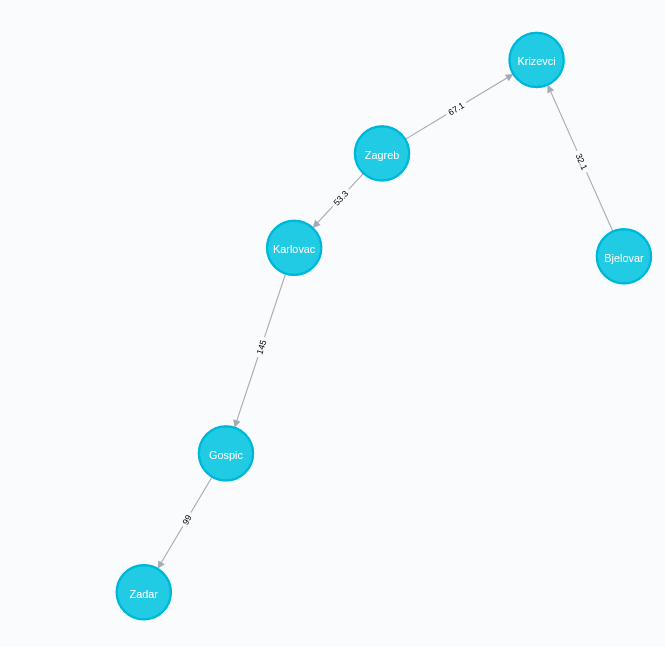
\includegraphics[scale=0.3]{zd-bjelovar}
    \caption{Najkraći put od Zadra do Bjelovara}
\end{figure}

\subsection{Upotreba Dijkstrinog algoritma}
Klasični primjer upotrebe ovog algoritma je računanje najbliže rute između dva udaljena mjesta.
U našoj grafovskoj bazi Dijkstrin algoritam primjenjujemo u istu svrhu. Ali nismo jedini. I u većim bazama koje sadrže gradove kao vrhove, a na bridovima im leži udaljenost također se koristi ovaj algoritam u izračunima. Tako primjerice \emph{Google Maps} koriste ovaj algoritam. On je doduše modificiran kako bi ga se ubrzalo, ali ideja ostaje ista. Još jedan primjer je i hrvatska softverska tvrtka \emph{Mireo}, poznata po svojim sustavima GPS navigacije koja se isto tako služi ubrzanim Dijkstrinim algoritmom. 
Kako u cestovnom prometu, algoritam se može koristiti i u zračnom prometu. Težine bridova tada su zračne udaljenosti, a vrhovi zračne luke.

Bitnu primjenu algoritam pronalazi i u sustavu telekomunikacijskih mreža.

Prethodno opisane primjene su poprilično očite. No, algoritam rješava i brojne druge probleme. 
Tako se primjerice koristi u društvenim mrežama. Većina mreža nudi opciju „prijatelja koje možda poznajemo”. Do tog rezultata dolaze primjenom Dijkstrinog algoritma na način da su vrhovi osobe, a težine bridova najčešće zajednički prijatelji.





\section{Najkraći put među svim parovima}
\section{Minimalno razapinjuće stablo}

Definirajmo najprije neke važne pojmove koji će nam pomoći u razumijevanju. 

\begin{definicija}
\emph{Podgraf} grafa $G = (V,E)$ je graf kojem su skup vrhova i skup bridova podskupovi od $V$ i $E$, redom. \emph{Inducirani podgraf} grafa $G$ induciran skupom $V'$ je podgraf $G' = (V', E')$, gdje se $E'$ sastoji od svih bridova od $G$ čija oba kraja leže u $V'$, dok je $V'$ neki zadani podskup od V. Razapinjući podgraf je podgraf oblika $G' = (V', E')$. 
\end{definicija}

\begin{definicija}
\emph{Šetnja} u grafu je niz $(v_0, e_1, v_1, e_2, v_2,\dotsc,e_n, v_n)$, gdje je $e_i = \{v_{i-1}, v_i\}$, 
za $i = 1,\dotsc,n$. Kažemo da je to šetnja od $v_0$ do $v_n$. Kažemo da je šetnja zatvorena ukoliko je $v_n = v_0$.
\emph{Staza} je šetnja u kojoj su svi bridovi različiti, dok je \emph{put} šetnja u kojoj su svi vrhovi različiti (osim
eventualno prvog i zadnjeg). Zatvoreni put zovemo \emph{ciklus}.
\end{definicija}

\begin{propozicija}
Za dva različita vrha $x,y$ grafa $G$ uvjeti da postoji šetnja, staza ili put između $x$ i $y$ su ekvivalentni.
\end{propozicija}

\begin{definicija}
Definiramo relaciju $\equiv$ na skupu vrhova $V$ grafa $G$: \\
$x \equiv y$ ako postoji put (ili staza ili šetnja) od $x$ do $y$. $\equiv$ je relacija ekvivalencije koja definira jednu particiju skupa $V$, te definiramo komponente povezanosti grafa kao podgrafove inducirane klasama ekvivalencije. Kažemo da je graf \emph{povezan}, ukoliko postoji samo jedna komponenta .
\end{definicija}

\begin{definicija}
\emph{Stablo} je povezan graf bez ciklusa. Šuma je graf bez ciklusa čije su komponente stabla. 
\end{definicija}

\begin{definicija}
Neka je G graf. \emph{Razapinjuća šuma} od $G$ je razapinjući podgraf of G koji je šuma. \emph{Razapinjuće stablo} od $G$ je razapinjući podgraf od $G$ koji je stablo. 
\end{definicija}

\begin{korolar}
Svaki povezani graf ima razapinjuće stablo. 
\end{korolar}

Sada kad smo se upoznali sa svim važnim definicijama i tvrdnjama, možemo konstruirati razapinjuće stablo grafa $G = (V,E)$:

%H kaže 'here', tj. tu počinje figura (onda latex stavlja tu figuru i tekst prije i poslije njega, inače može doći do miješanja)
\begin{croatianalgorithm}[H]
  \caption{Razapinjuće stablo}
  \begin{algorithmic}[1]
    \STATE $S = \emptyset$
    \WHILE{je graf $(V,S)$ nepovezan}
      \STATE nađi brid $e$ koji povezuje vrhove u različitim komponentama
      \STATE dodaj $e$ u $S$
    \ENDWHILE
    \RETURN{$(V,S)$}
  \end{algorithmic}
\end{croatianalgorithm}

Međutim, što ako želimo naći povezani razapinjući podgraf s minimalnom težinom (tj. sumom težina bridova podgrafa)? Takav podgraf mora biti stablo, inače bismo mogli izbrisati neki brid, smanjujući težinu, a ne pokvarivši povezanost. 

\begin{definicija}
\emph{Minimalno razapinjuće stablo} (MST) je stablo koje povezuje sve vrhove nekog (težinskog) grafa, pri čemu je ukupna suma težina svih bridova minimalna. 
\end{definicija}
Najpoznatiji algoritmi za pronalaženje MST-a su \emph{Kruskalov} i \emph{Primov}. 

\subsection{Kruskalov algoritam}

Neka je $G = (V, E)$ povezan graf, $\omega$ nenegativna težinska funkcija na $E$. Tada Kruskalov algoritam možemo ovako zapisati:

\begin{croatianalgorithm}[H]
  \caption{Kruskalov algoritam}
  \begin{algorithmic}[1]
    \STATE $S = \emptyset$
    \WHILE{$(V, S)$ nije povezan}
      \STATE odaberi brid $e \in E\setminus S$ minimalne težine, takav da $S \cup \{e\}$ nema ciklus
      \STATE $S = S \cup\{e\}$
    \ENDWHILE
    \RETURN{$(V,S)$}
  \end{algorithmic}
\end{croatianalgorithm}


Dakle, u svakom koraku odabiremo brid najmanje težine, takav da njegovo ubacivanje ne stvara ciklus. Mana ovog algoritma je to što nije baš jednostavno pronaći brid minimalne težine koji spaja vrhove iz različitih komponenti. Stoga postoji izmijenjen Kruskalov algoritam, gdje u svakom koraku biramo brid najmanje težine koji spaja neki vrh s nekim vrhom koji još nije spojen. Taj algoritam se naziva \emph{Primov algoritam}.

\subsection{Primov algoritam}

Neka je $G = (V, E)$, $|V| = n$, povezan graf i $\omega$ nenegativna težinska funkcija na $E$. 
Primov algoritam možemo ovako zapisati:

\begin{croatianalgorithm}[H]
  \caption{Primov algoritam}
  \begin{algorithmic}[1]
    \STATE Odaberemo $v_0 \in V$ i definiramo $T = \{v_0\}$, $S = V\setminus{\{v_0\}}$, $F = \emptyset$
    \WHILE{$|F| < n-1$}
      \STATE odaberi brid $e = \{v,w\}$ iz $E$ minimalne težine, takav da je $v$ iz $T$, $w$ iz $S$
      \STATE $T = T \cup \{w\}$, $F = F \cup \{e\}$, $S = S \setminus \{w\}$
    \ENDWHILE
    \RETURN{$(V,F)$}
  \end{algorithmic}
\end{croatianalgorithm}

Kako je Primov algoritam poboljšani Kruskalov algoritam, koristeći njega ćemo pokazati na našoj bazi gradova kako pronaći minimalno razapinjuće stablo. Naglasimo da minimalno stablo ne mora biti jedinstveno, ali težina svakog minimalnog stabla uistinu je minimalna, tj. jedinstvena. Ovaj algoritam zahtjeva odabir proizvoljnog vrha za početak, a s obzirom na to da je Zagreb glavni grad Hrvatske, odaberimo upravo njega. Ovaj algoritam ćemo provesti u koracima \emph{while} petlje iznad, stoga najprije uzimamo $v_0 = \text{ Zagreb}$, pa je $T = \{\text{Zagreb}\}$ te je  $S = V\setminus{\{v_0\}}$, a $F = \emptyset$, gdje je $V$ skup svih vrhova našeg grafa, tj. $29$ gradova ($n = 29$). Prateći gornji algoritam, pogledajmo s kojim gradovima je grad Zagreb povezan. 

%H kaze 'here' kao uvdje, T je top of the page
\begin{figure}[H]
\texttt{MATCH (a {name:'Zagreb'})-[:CONNECTION]-(b) RETURN a,b;}
\caption{Zagreb i njegovi susjedi}
\begin{center}
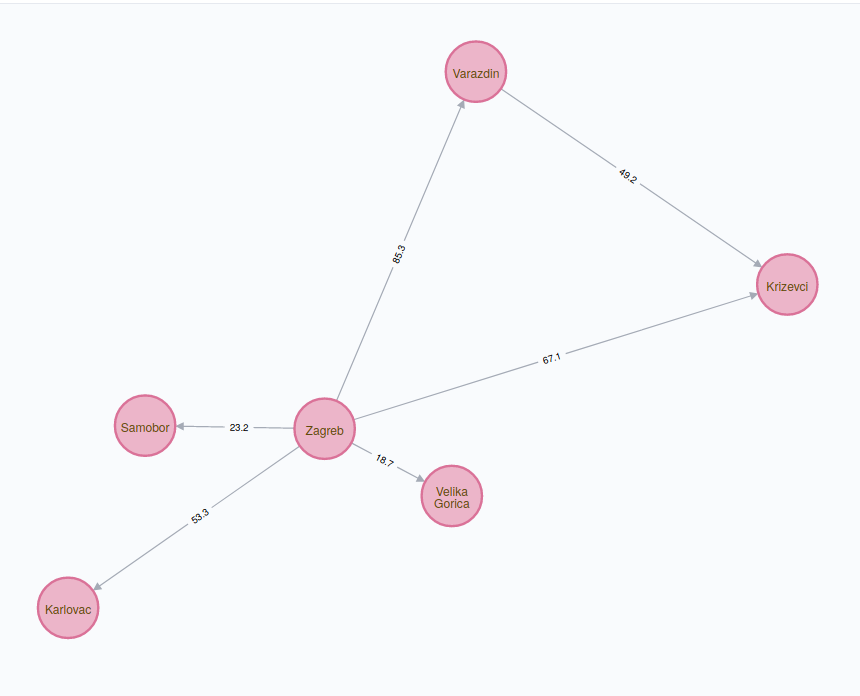
\includegraphics[scale=0.3]{Zagreb}
\end{center}
\end{figure}

Sada odabiremo brid minimalne težine koji je povezan sa Zagrebom, stoga biramo brid koji povezuje Zagreb i Veliku
Goricu (težine $18.7$). Pogledajmo sada stanje naših skupova:
\newline

\begin{tabular}{|l|l|}
\hline
 $T$ &  Zagreb, Velika Gorica\\ \hline
 $F$ &  $\{\{$ Zagreb, Velika Gorica $\}\}$\\ \hline
\end{tabular}
\newline

Algoritam provodimo sve dok je $|F| < n-1 = 28$, stoga nastavljamo. Sada promatramo sve susjede od Zagreba i Velike Gorice i
među neodabranim bridovima biramo onaj minimalne težine. 

\begin{figure}[H]
\caption{Zagreb, Velika Gorica i njihovi susjedi}
\begin{center}
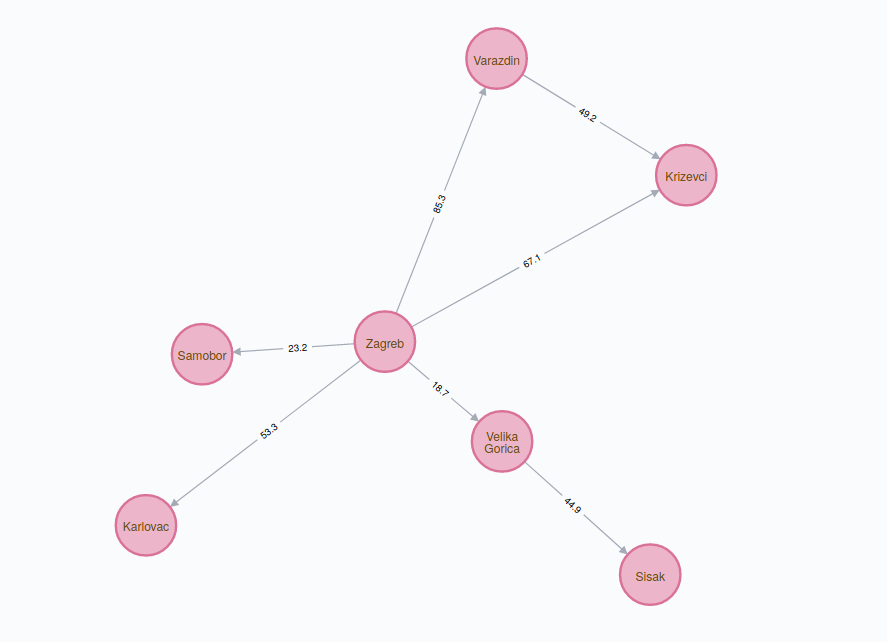
\includegraphics[scale=0.3]{Zg-VG}
\end{center}
\end{figure}

Vidimo da ćemo idući brid biti onaj koji povezuje Zagreb i Samobor čija je težina $23.2$. Redom dalje ćemo odabirati bridove minimalne težine kao što je prikazano na tablici niže. Svaki odabrani brid ima svoju težinu $\omega$. Dobivenom MST-u računamo ukupnu težinu tako što zbrajamo težine svih bridova u tom stablu.
\begin{equation}
    \sum_{v \in V} \omega(v) = 1684
\end{equation}
\newline
\begin{table}[H]
\centering
\begin{tabular}{|l|l|l|} 
\hline
\textbf{T = posjećeni vrhovi}          & \textbf{F = posjećeni bridovi}                        & \textbf{S = neposjećeni vrhovi}                        \\ 
\hline
$v_0=$ \{Zagreb\}                      & $\emptyset$                                           & $S = V \setminus v_0 = V \setminus \{\text{Zagreb}\}$  \\ 
\hline
$T = T \cup \{\text{Velika Gorica}\}$  & $F = F \cup \{\text{Zagreb, Velika Gorica}\}$         & $S = S \setminus \{\text{Velika Gorica}\}$             \\ 
\hline
$T = T \cup \{\text{Samobor}\}$        & $F = F \cup \{\text{Zagreb, Samobor}\}$               & $S = S \setminus \{\text{Samobor}\}$                   \\ 
\hline
$T = T \cup \{\text{Sisak}\}$          & $F = F \cup \{\text{Velika Gorica, Sisak}\}$          & $S = S \setminus \{\text{Sisak}\}$                     \\ 
\hline
$T = T \cup \{\text{Karlovac}\}$       & $F = F \cup \{\text{Zagreb, Karlovac}\}$              & $S = S \setminus \{\text{Karlovac}\}$                  \\ 
\hline
$T = T \cup \{\text{Križevci}\}$       & $F = F \cup \{\text{Zagreb, Križevci}\}$              & $S = S \setminus \{\text{Križevci}\}$                  \\ 
\hline
$T = T \cup \{\text{Bjelovar}\}$       & $F = F \cup \{\text{Križevci, Bjelovar}\}$            & $S = S \setminus \{\text{Bjelovar}\}$                  \\ 
\hline
$T = T \cup \{\text{Koprivnica}\}$     & $F = F \cup \{\text{Križevci, Koprivnica}\}$          & $S = S \setminus \{\text{Koprivnica}\}$                \\ 
\hline
$T = T \cup \{\text{Varaždin}\}$       & $F = F \cup \{\text{Koprivnica, Varaždin}\}$          & $S = S \setminus \{\text{Varaždin}\}$                  \\ 
\hline
$T = T \cup \{\text{Čakovec}\}$        & $F = F \cup \{\text{Varaždin, Čakovec}\}$             & $S = S \setminus \{\text{Čakovec}\}$                   \\ 
\hline
$T = T \cup \{\text{Virovitica}\}$     & $F = F \cup \{\text{Koprivnica, Virovitica}\}$        & $S = S \setminus \{\text{Virovitica}\}$                \\ 
\hline
$T = T \cup \{\text{Nova Gradiška}\}$  & $F = F \cup \{\text{Sisak, Nova Gradiška}\}$          & $S = S \setminus \{\text{Nova Gradiška}\}$             \\ 
\hline
$T = T \cup \{\text{Slavonski Brod}\}$ & $F = F \cup \{\text{Nova Gradiška, Slavonski Brod}\}$ & $S = S \setminus \{\text{Slavonski Brod}\}$            \\ 
\hline
$T = T \cup \{\text{Đakovo}\}$         & $F = F \cup \{\text{Slavonski Brod, Đakovo}\}$        & $S = S \setminus \{\text{Đakovo}\}$                    \\ 
\hline
$T = T \cup \{\text{Vinkovci}\}$       & $F = F \cup \{\text{Đakovo, Vinkovci}\}$              & $S = S \setminus \{\text{Vinkovci}\}$                  \\ 
\hline
$T = T \cup \{\text{Vukovar}\}$        & $F = F \cup \{\text{Vinkovci, Vukovar}\}$             & $S = S \setminus \{\text{Vukovar}\}$                   \\ 
\hline
$T = T \cup \{\text{Osijek}\}$         & $F = F \cup \{\text{Vukovar, Osijek}\}$               & $S = S \setminus \{\text{Osijek}\}$                    \\ 
\hline
$T = T \cup \{\text{Rijeka}\}$         & $F = F \cup \{\text{Karlovac, Rijeka}\}$              & $S = S \setminus \{\text{Rijeka}\}$                    \\ 
\hline
$T = T \cup \{\text{Pula}\}$           & $F = F \cup \{\text{Rijeka, Pula}\}$                  & $S = S \setminus \{\text{Pula}\}$                      \\ 
\hline
$T = T \cup \{\text{Gospić}\}$         & $F = F \cup \{\text{Karlovac, Gospić}\}$              & $S = S \setminus \{\text{Gospić}\}$                    \\ 
\hline
$T = T \cup \{\text{Zadar}\}$          & $F= F \cup \{\text{Gospić, Zadar}\}$                  & $S = S \setminus \{\text{Zadar}\}$                     \\ 
\hline
$T = T \cup \{\text{Šibenik}\}$        & $F = F \cup \{\text{Zadar, Šibenik}\}$                & $S = S \setminus \{\text{Šibenik}\}$                   \\ 
\hline
$T = T \cup \{\text{Kaštela}\}$        & $F = F \cup \{\text{Šibenik, Kaštela}\}$                & $S = S \setminus \{\text{Kaštela}\}$                  \\ 
\hline
$T = T \cup \{\text{Split}\}$          & $F = F \cup \{\text{Kaštela, Split}\}$                 & $S = S \setminus \{\text{Split}\}$                     \\ 
\hline
$T = T \cup \{\text{Sinj}\}$           & $F = F \cup \{\text{Split, Sinj}\}$                   & $S = S \setminus \{\text{Sinj}\}$                      \\ 
\hline
$T = T \cup \{\text{Knin}\}$           & $F = F \cup \{\text{Šibenik, Knin}\}$                 & $S = S \setminus \{\text{Knin}\}$                      \\ 
\hline
$T = T \cup \{\text{Imotski}\}$        & $F = F \cup \{\text{Sinj, Imotski}\}$                 & $S = S \setminus \{\text{Imotski}\}$                   \\ 
\hline
$T = T \cup \{\text{Makarska}\}$       & $F = F \cup \{\text{Imotski, Makarska}\}$             & $S = S \setminus \{\text{Makarska}\}$                  \\ 
\hline
$T = T \cup \{\text{Dubrovnik}\}$      & $F = F \cup \{\text{Makarska, Dubrovnik}\}$           & $S = S \setminus \{\text{Dubrovnik}\} = \emptyset$                 \\
\hline
\end{tabular}
\end{table}
Dakle, dobiveno minimalno razapinjuće stablo sastoji se od dvih $29$ vrhova te bridova iz dobivenog skupa $F$. Provjerimo sada kako izgleda minimalno razapinjuće stablo koje dobijemo koristeći se sljedećim \emph{Cypher} upitom:\\
\newline
\texttt{MATCH path = (n:City {name:"Zagreb"})-[:MINST*]-()}\\
\texttt{WITH relationships(path) AS rels}\\
\texttt{UNWIND rels AS rel}\\
\texttt{WITH DISTINCT rel AS rel} \\
\texttt{RETURN startNode(rel).name AS source, endNode(rel).name AS destination,}\\
\texttt{rel.distance AS cost;}\\
Nakon toga upitom 
\texttt{MATCH (n) RETURN n;}
dobijemo sliku niže, gdje se nalazi naš graf kojem su dodani bridovi koji će činiti MST. Pogledamo li malo bolje, to su upravo bridovi koje smo i mi dobili Primovim algoritmom, stoga je težina ovog grafa također $1684$, što potvrđuje činjenicu da smo uistinu dobili minimalno razapinjuće stablo. \\

\begin{figure}[H]
\caption{Minimalno razapinjuće stablo}
\begin{center}
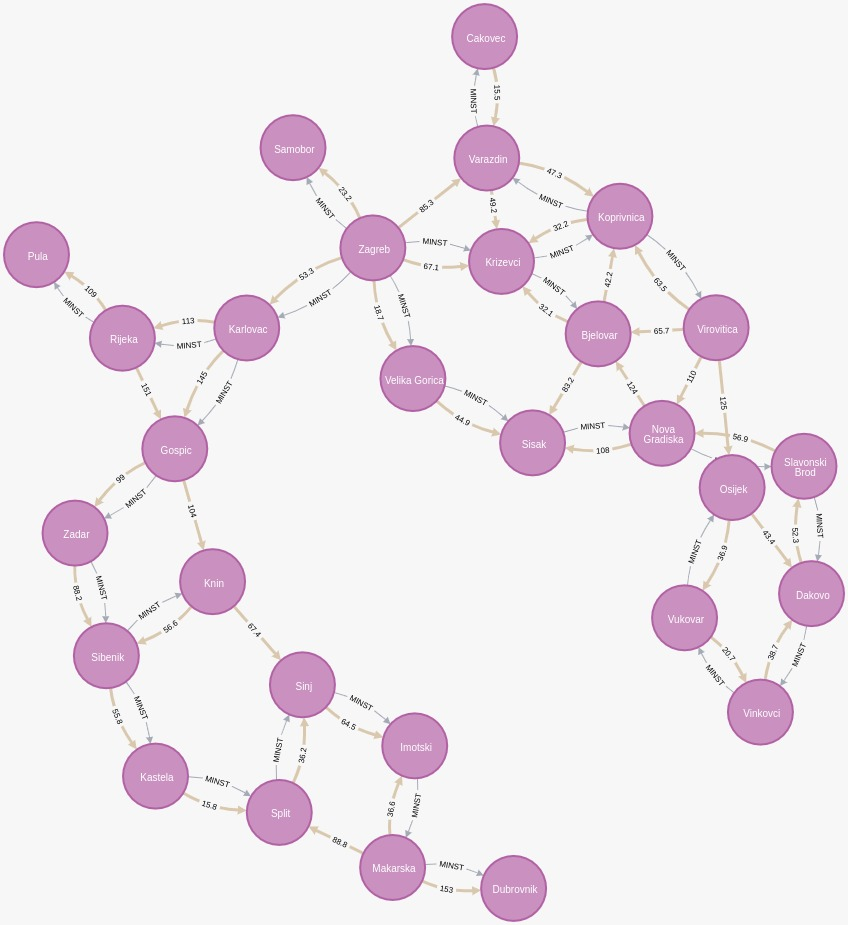
\includegraphics[scale=0.4]{MST}
\end{center}
\end{figure}

\subsection{Primjena minimalnog razapinjućeg stabla}
A zašto je ovo korisno? Recimo da se moraju postaviti telekomunikacijski kabeli između svaka dva grada. Telekomunikacijska tvrtka dakako razmišlja o optimalnom ulaganju, gdje bi potrošili što manje novca, a istovremeno uspjeli na neki način povezati sve gradove (između svaka dva grada postoji telekomunikacijski kabel, makar preko nekog drugog grada). Pronalaženjem minimalnog razapinjućeg stabla ova tvrtka će dobiti savršen plan za minimiziranje svog troška. 



\end{document}
